%%%%%%%%%%%%%%%%%%%%%%%%%%%%%%%%%%%%%%%%%
% Beamer Presentation
% LaTeX Template
% Version 1.0 (10/11/12)
%
% This template has been downloaded from:
% http://www.LaTeXTemplates.com
%
% License:
% CC BY-NC-SA 3.0 (http://creativecommons.org/licenses/by-nc-sa/3.0/)
%
%%%%%%%%%%%%%%%%%%%%%%%%%%%%%%%%%%%%%%%%%

%----------------------------------------------------------------------------------------
%	PACKAGES AND THEMES
%----------------------------------------------------------------------------------------

\documentclass{beamer}

\mode<presentation> {

% The Beamer class comes with a number of default slide themes
% which change the colors and layouts of slides. Below this is a list
% of all the themes, uncomment each in turn to see what they look like.

%\usetheme{default}
%\usetheme{AnnArbor}
%\usetheme{Antibes}
%\usetheme{Bergen}
%\usetheme{Berkeley}
%\usetheme{Berlin}
%\usetheme{Boadilla}
%\usetheme{CambridgeUS}
%\usetheme{Copenhagen}
%\usetheme{Darmstadt}
%\usetheme{Dresden}
%\usetheme{Frankfurt}
%\usetheme{Goettingen}
%\usetheme{Hannover}
%\usetheme{Ilmenau}
%\usetheme{JuanLesPins}
%\usetheme{Luebeck}
\usetheme{Madrid}
%\usetheme{Malmoe}
%\usetheme{Marburg}
%\usetheme{Montpellier}
%\usetheme{PaloAlto}
%\usetheme{Pittsburgh}
%\usetheme{Rochester}
%\usetheme{Singapore}
%\usetheme{Szeged}
%\usetheme{Warsaw}

% As well as themes, the Beamer class has a number of color themes
% for any slide theme. Uncomment each of these in turn to see how it
% changes the colors of your current slide theme.

%\usecolortheme{albatross}
%\usecolortheme{beaver}
%\usecolortheme{beetle}
%\usecolortheme{crane}
%\usecolortheme{dolphin}
%\usecolortheme{dove}
%\usecolortheme{fly}
%\usecolortheme{lily}
%\usecolortheme{orchid}
%\usecolortheme{rose}
%\usecolortheme{seagull}
%\usecolortheme{seahorse}
%\usecolortheme{whale}
%\usecolortheme{wolverine}

%\setbeamertemplate{footline} % To remove the footer line in all slides uncomment this line
%\setbeamertemplate{footline}[page number] % To replace the footer line in all slides with a simple slide count uncomment this line

%\setbeamertemplate{navigation symbols}{} % To remove the navigation symbols from the bottom of all slides uncomment this line
}
\usepackage[markup=nocolor]{changes}
\usepackage{graphicx} % Allows including images
\usepackage{booktabs} % Allows the use of \toprule, \midrule and \bottomrule in tables

%----------------------------------------------------------------------------------------
%	TITLE PAGE
%----------------------------------------------------------------------------------------

\title[First-past-the-post election system]{Evaluating the NRW 2013, 2017, 2019 with the first-past-the-post election system} % The short title appears at the bottom of every slide, the full title is only on the title page

\author{L. da Cunha Melo \& S. Reisinger} % Your name
\institute[] % Your institution as it will appear on the bottom of every slide, may be shorthand to save space
{
TU Wien \\ % Your institution for the title page
\medskip
\textit{} % Your email address
}
\date{\today} % Date, can be changed to a custom date

\begin{document}

\begin{frame}
\titlepage % Print the title page as the first slide
\end{frame}

\begin{frame}
\frametitle{Overview} % Table of contents slide, comment this block out to remove it
\tableofcontents % Throughout your presentation, if you choose to use \section{} and \subsection{} commands, these will automatically be printed on this slide as an overview of your presentation
\end{frame}

%----------------------------------------------------------------------------------------
%	PRESENTATION SLIDES
%----------------------------------------------------------------------------------------

\section{Introduction} 
% With the US election coming up this November we thought it is interesting how the results and the Distribution lower house of the USA and Au

\begin{frame}
\frametitle{Current House of the Representatives Map}
\begin{figure}[h]
\centering
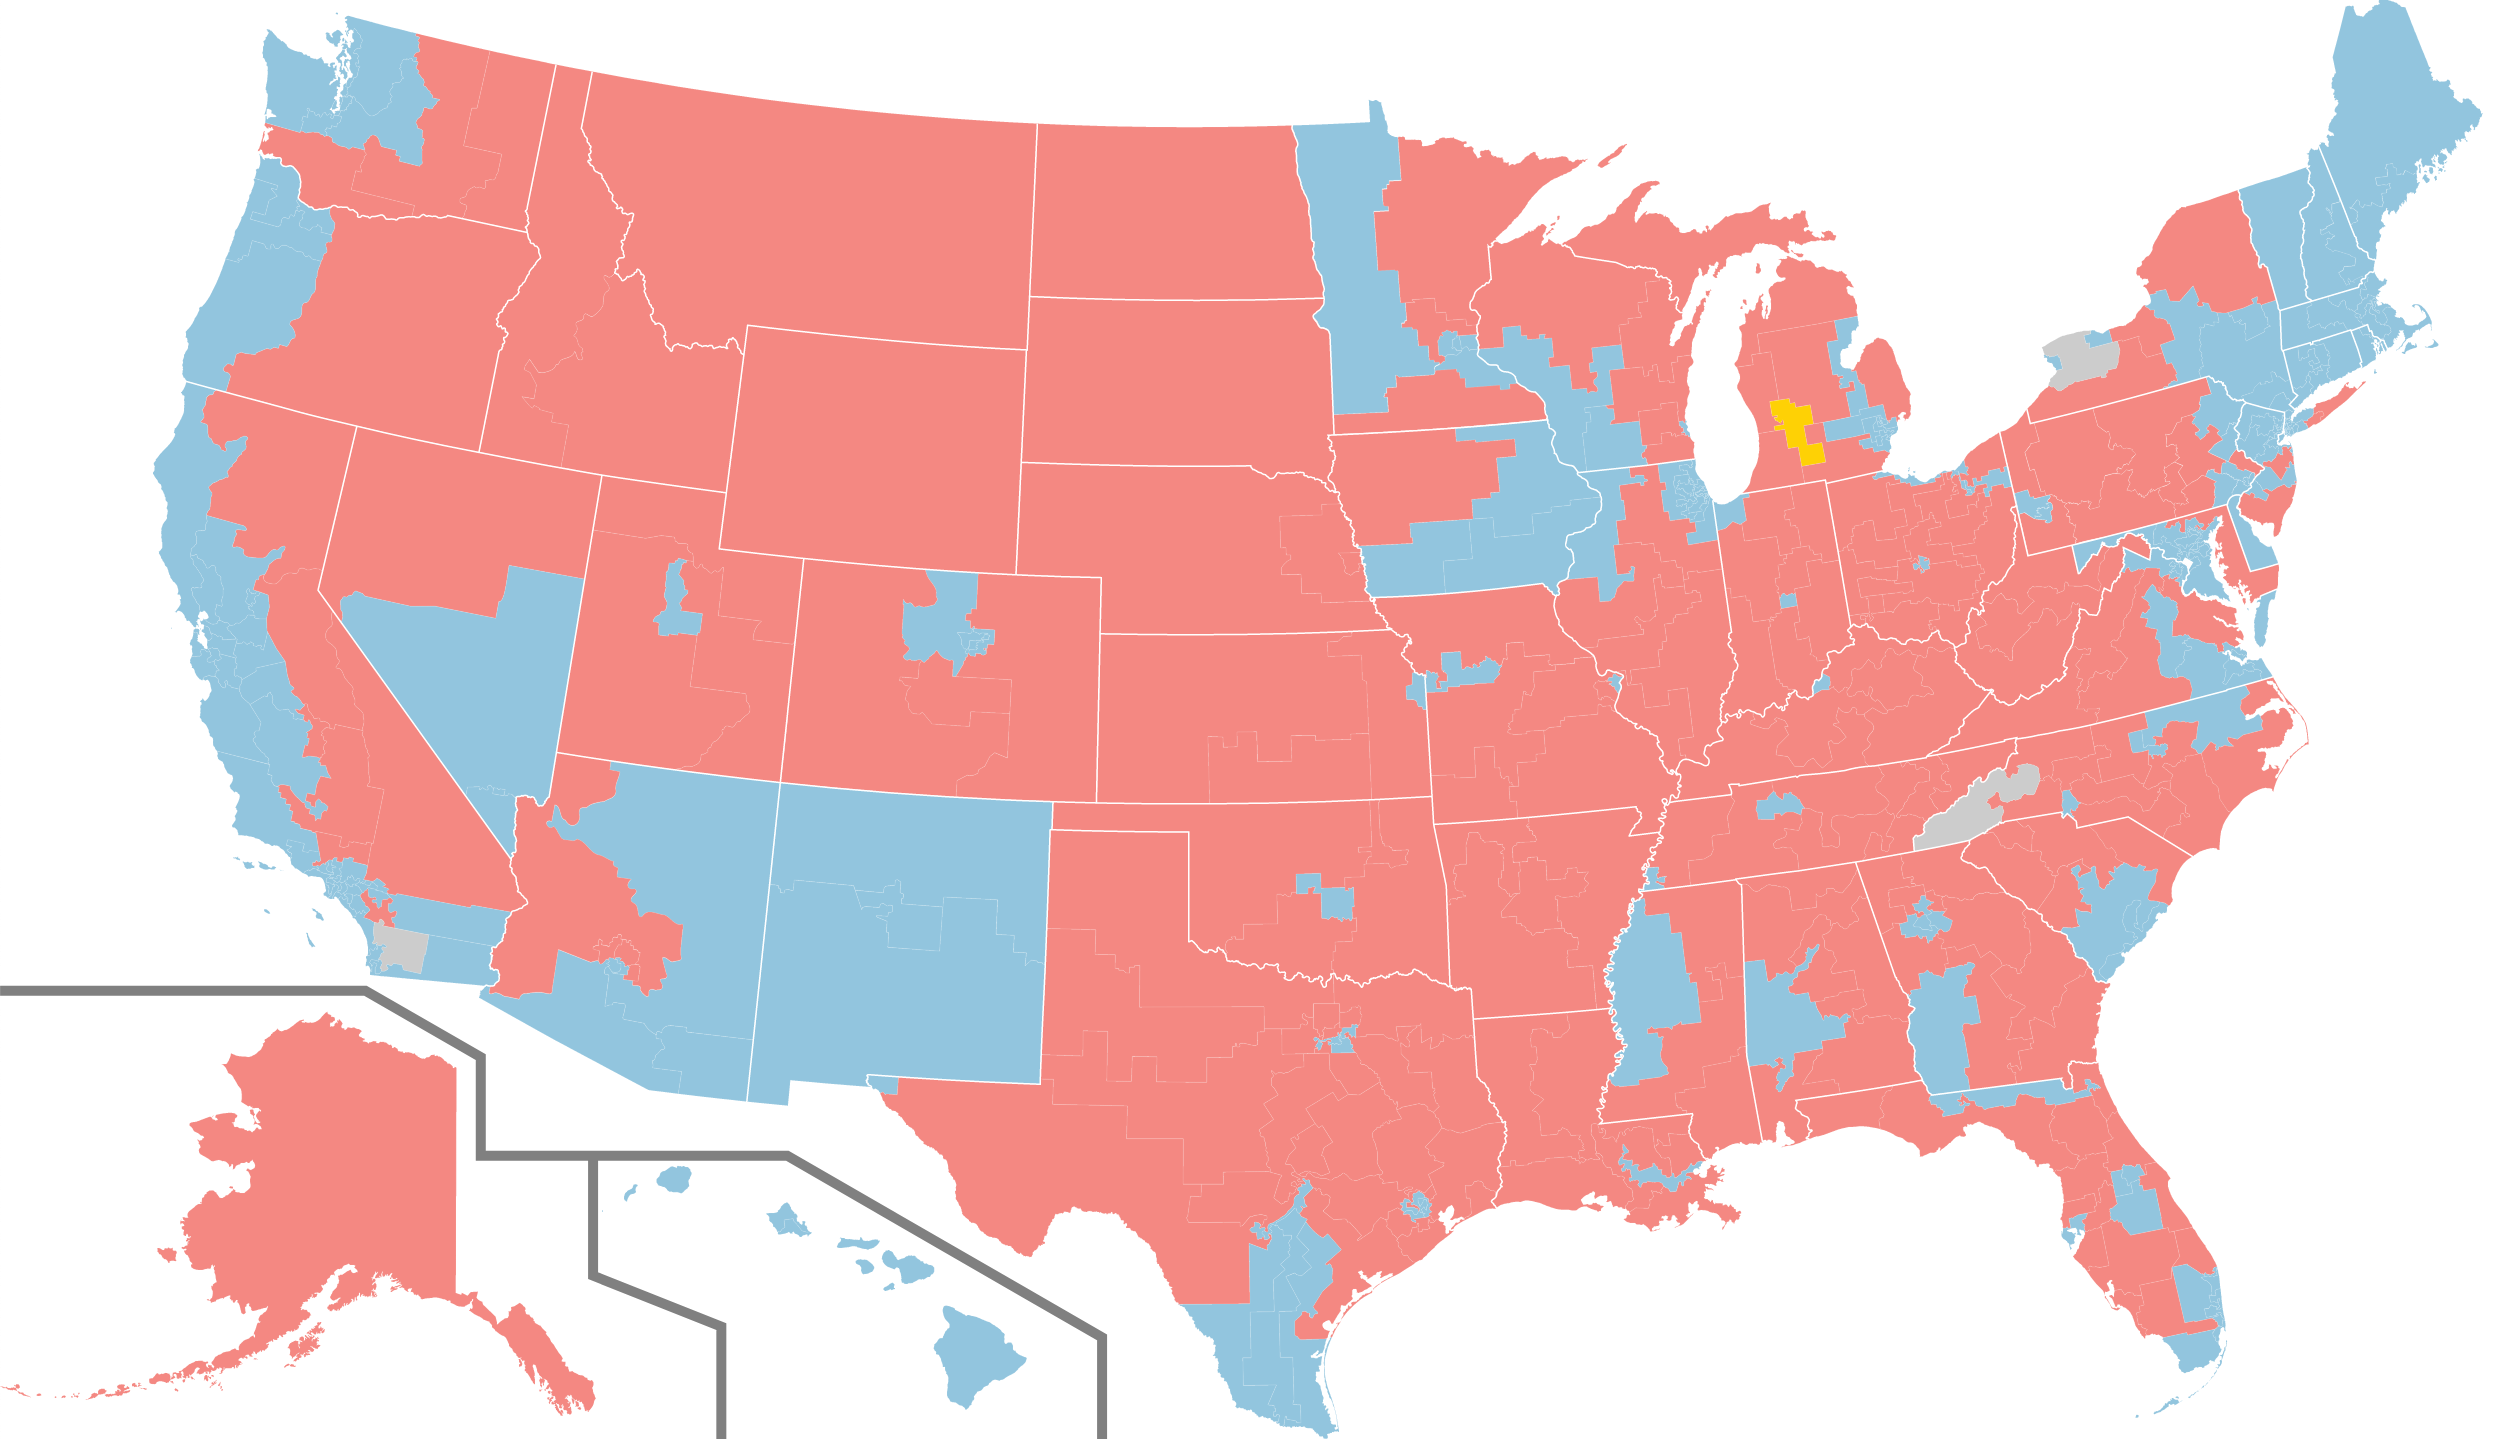
\includegraphics[width=4cm]{images/us_map.png}
\caption{House composition by district of the USA}\label{fig:mapOfResults}
\bigbreak
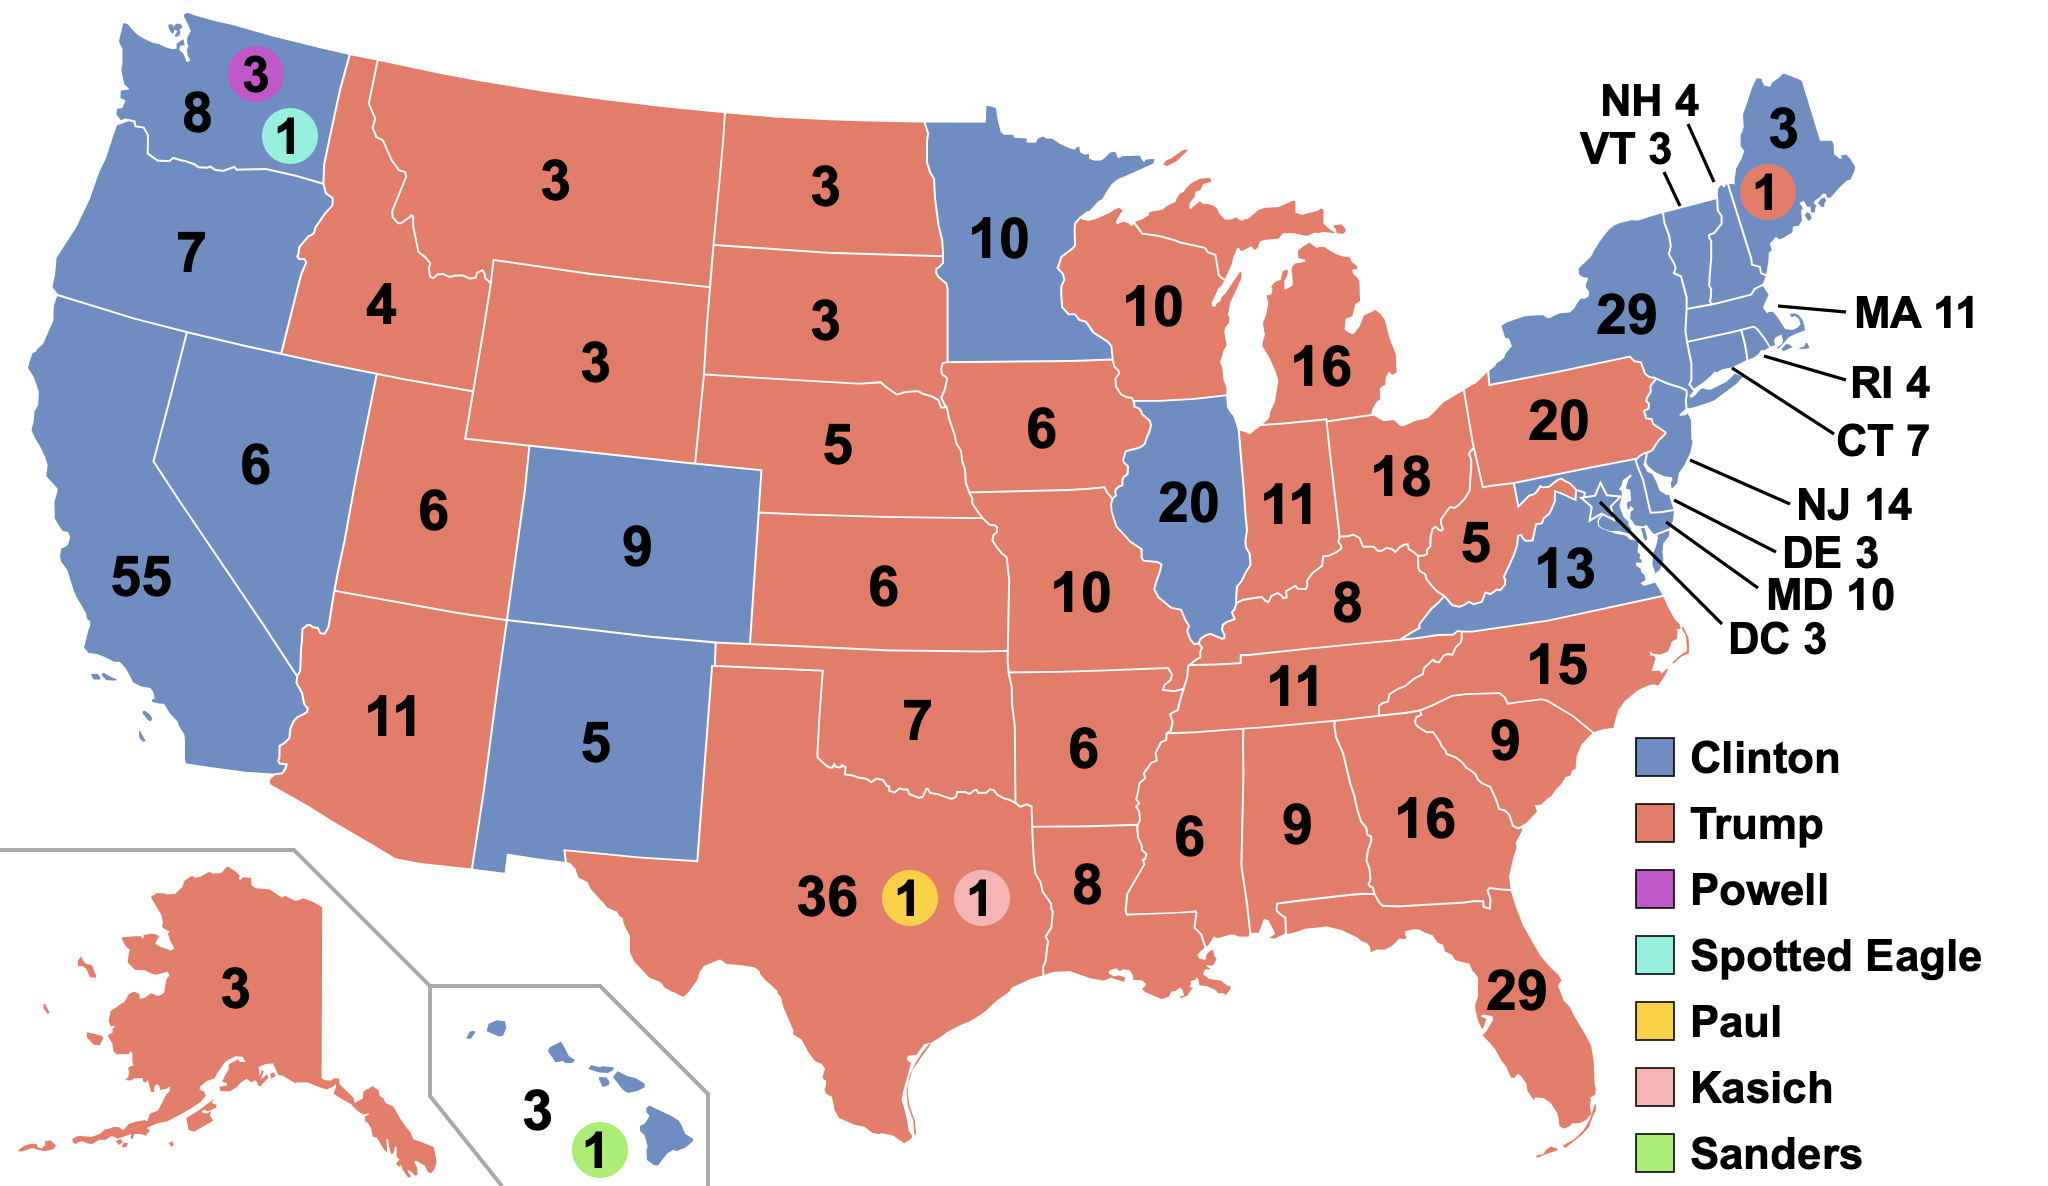
\includegraphics[width=4cm]{images/US_2016_Election.png}
\caption{Map of the 2016 United States presidential election}\label{fig:mapOfResultsPresidential}
\end{figure}
% In the US they do not vote for a Presidential Candidate but for members of the United States Electoral College. The Electoral College will vote then Vote for the President
\end{frame}

\begin{frame}
\frametitle{First-past-the-post Voting vs Proportional Representation}
% The most common method used in U.S. elections is the first-past-the-post system, where the highest-polling candidate wins the election. Under this system, a candidate only requires a plurality of votes to win, rather than an outright majority.
\begin{itemize}
\item First-past-the-post: The candidate with the most votes wins the election
\begin{itemize}
    \item Example: let there be 9 candidates (candidates $A$ through $I$)
    \item Candidate $A$ gets 16\% of the votes, while candidate $B$ gets $14\%$ and candidates $C-I$ each get 10\%
    \item Candidate $A$ wins despite 84\% of people voting on other candidates
\end{itemize}

% FPTP is most often criticized for its failure to reflect the popular vote in the number of seats awarded to competing parties. But it is better at represent all parts of the country. It gives equal power to dense populated areas as to to 
% https://en.wikipedia.org/wiki/First-past-the-post_voting#Criticisms

\item Proportional Representation: The candidate with at least 50\%+1 of votes wins the election
\begin{itemize}
    \item Consider situation of the previous example
    \item Candidates $A$ and $B$ go to second round (or build a coalition)
\end{itemize}

% PR tries to resolve the unfairness of majoritarian and plurality voting systems where the largest parties receive an "unfair" "seat bonus" and smaller parties are disadvantaged and are always under-represented

\end{itemize}

\begin{figure}
    \centering
    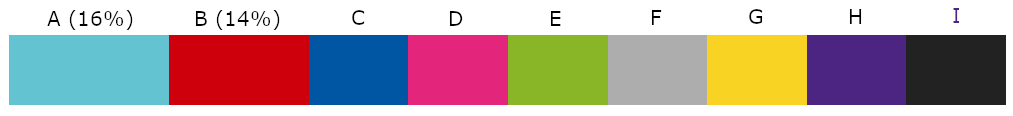
\includegraphics[width=0.9\textwidth]{images/partiesExample.png}
\end{figure}

\end{frame}

\begin{frame}{Questions}
    %\centerline{\Huge{\color{red} TODO}}
    \begin{itemize}
        \item How would the Austrian government and lower house look like if we used the US Election System?
        \item Can we show examples for the advantages and disadvantages of the First Past The Post election system if we use it to evaluate the Austrian election?
    \end{itemize}
\end{frame}

\section{Data} 
\begin{frame}
\frametitle{Data set}
\begin{itemize}
\item Maps: \href{https://www.data.gv.at}{Verwaltungsgrenzen Österreich} by Districts (Bezirke) and Municipalitiess (Gemeinden)
\item Results of the NRW 2019: Provided in Exercise 2
\item Results of the NRWs 2013 and 2017: \href{https://www.data.gv.at}{data.gv.at}
\item Wahlkreise from \href{https://www.bmi.gv.at/412/Nationalratswahlen/Wahlkreiseinteilung.aspx}{bmi.gv.at}
\end{itemize}

\end{frame}

\begin{frame}
\frametitle{Problems with Data Sets}
% There are inconsistencies in the spelling through the two data sets.
% All changes were made in code only because so the r
\begin{itemize}
\item District inconsistencies:
    \begin{itemize}
    \item Stadt: "Innsbruck-Stadt", "Klagenfurt Stadt", "Wiener Neustadt(Stadt)"
    \item Land: "Linz-Land", "Klagenfurt Land", "Sankt Pölten(Land)"
    \end{itemize}
\item Municipalities merging:
% ISO Numbers were updated over time and some of the villages were merged together.
    \begin{itemize}
        \item iso:
        \begin{itemize}
            \item 41625, 41340: 41628 (Schönegg $\rightarrow$ Vorderweißenbach)
            \item 41301, 41335: 41346 ((Afiesl, St. Stefan am Walde) $\rightarrow$ St. Stefan-Afiesl)
            \item 40803, 40819: 40835 (Bruck-Waasen $\rightarrow$ Peuerbach)
            \item 41310, 41302: 41345 (Ahorn $\rightarrow$ Helfenberg)
        \end{itemize}
    \end{itemize}
\item More (other) inconsistencies:
    \begin{itemize}
    \item Umgebung: "Hartberg Umgebung", "Eisenstadt - Umgebung"
    \end{itemize}
\end{itemize}
\end{frame}





\begin{frame}
\frametitle{Assumption and Simplifications}
\begin{itemize}
% Due to the fact that we use a different Election System for decades now. Therefore the results have to be taken with a grain of salt.
\item Election: Executive branch
% In Austria we do not vote for the government directly therefore we used the results of the Nationalratswahl 2019. And interpreted it like they would vote for the lead candidate ("Spitzenkandidat")
    \begin{itemize}
    \item Districts instead of the States
    % We did not use the states of Austria because there are too little and used the counties instead. 
    % Wahlkreise are drawn and the Number of Mandate are 
    \item Mandate instead of the electoral college
    % Like the Members of the Electoral College the Mandate in Austria are 
    \item No faithless electors
% For the Presidential election we ignoring Faithless electors. Member of the United States Electoral College who does not vote for the presidential or vice presidential candidate for whom they had pledged to vote. In the history of the united states it never changed the result of the election.
    \end{itemize}
\item Election: Legislative branch (Lower House)
\begin{itemize}
    \item Wahlkreise instead of the congressional districts
    % We did not use the states of Austria because there are too little and used the counties instead. 
    % The main problem with the counties is that they have big differences in size. 
    \end{itemize}
\item \deleted{Election: Legislative branch (Upper House)}
% There is no practical way in interpreting the given data to simulate these elections. The main problem is that in the USA it is not uncommon for two candidates to be elected from two different political parties.
\end{itemize}
\end{frame}

\section{Implementation} 
\begin{frame}
\frametitle{Tools/Languages Used}
\begin{itemize}
\item HTML + CSS % (+ Font Awesome)
\item JavaScript + D3 
% D3: Graphics; jquery: to triggering dropdown menu
% No php: This makes it possible to host on github.io
%\item Hosting: github.io
%\item IDE: Webstorm
\end{itemize}
\end{frame}


\section{Results} 

\begin{frame}
\frametitle{Results over the years}
\begin{figure}[h]
  \centering
  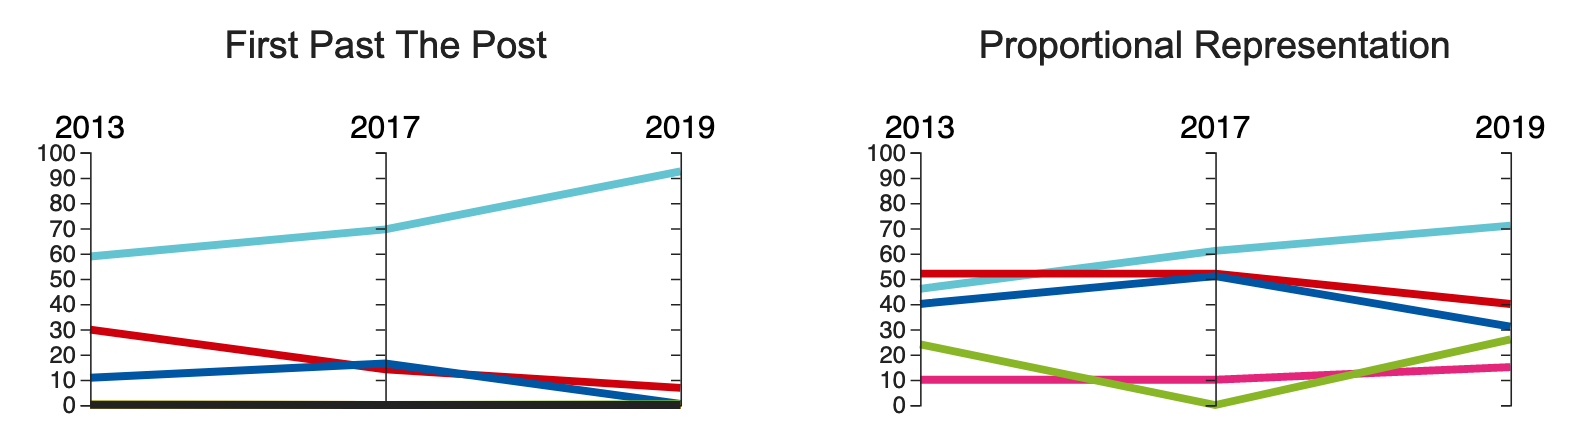
\includegraphics[width=0.9\linewidth]{images/paralellCoordinates.png} %TODO edit here
  \caption{\label{fig:mapOfResults} Map of Results}
\end{figure}
\end{frame}


\begin{frame}
\frametitle{Results by Municipalities (Gemeinden)}
\begin{figure}[h]
  \centering
  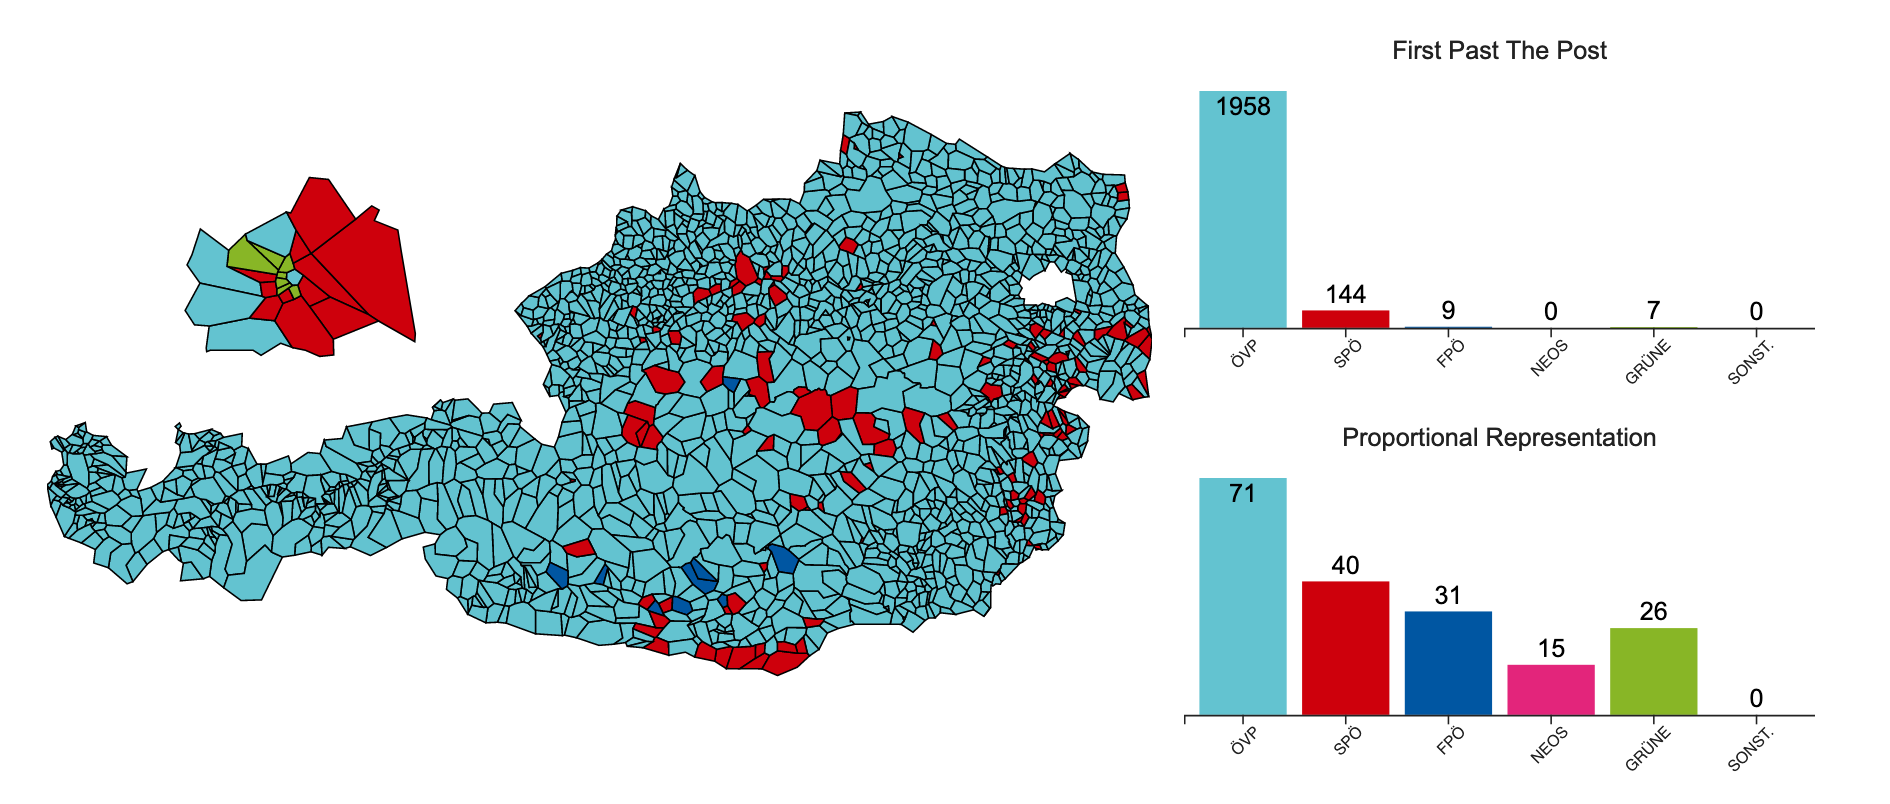
\includegraphics[width=0.9\linewidth]{images/mapbyGemeinden.png} %TODO edit here
  \caption{\label{fig:mapOfResults} Map of Results}
\end{figure}
\end{frame}

\begin{frame}
\frametitle{Results by Districts (Bezirke)}
\begin{figure}[h]
  \centering
  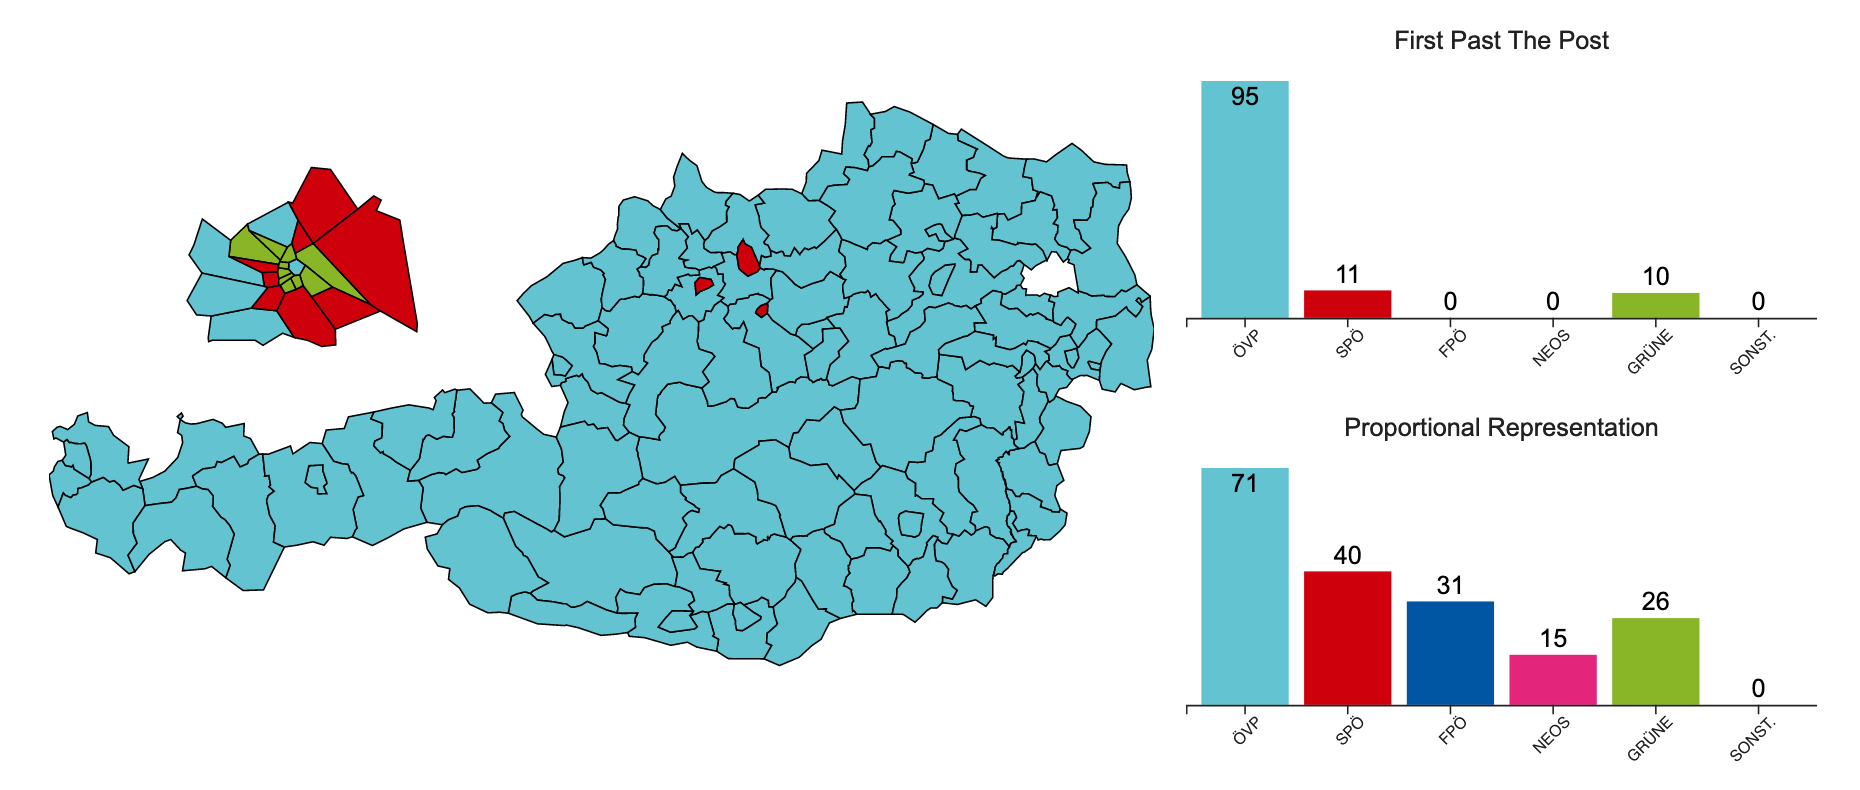
\includegraphics[width=0.9\linewidth]{images/mapbyBezirken.png}
  \caption{\label{fig:mapOfResults} Map of Results}
\end{figure}
\end{frame}


\begin{frame}
\frametitle{Results by Electoral District (Wahlkreis)}
\begin{figure}[h]
  \centering
  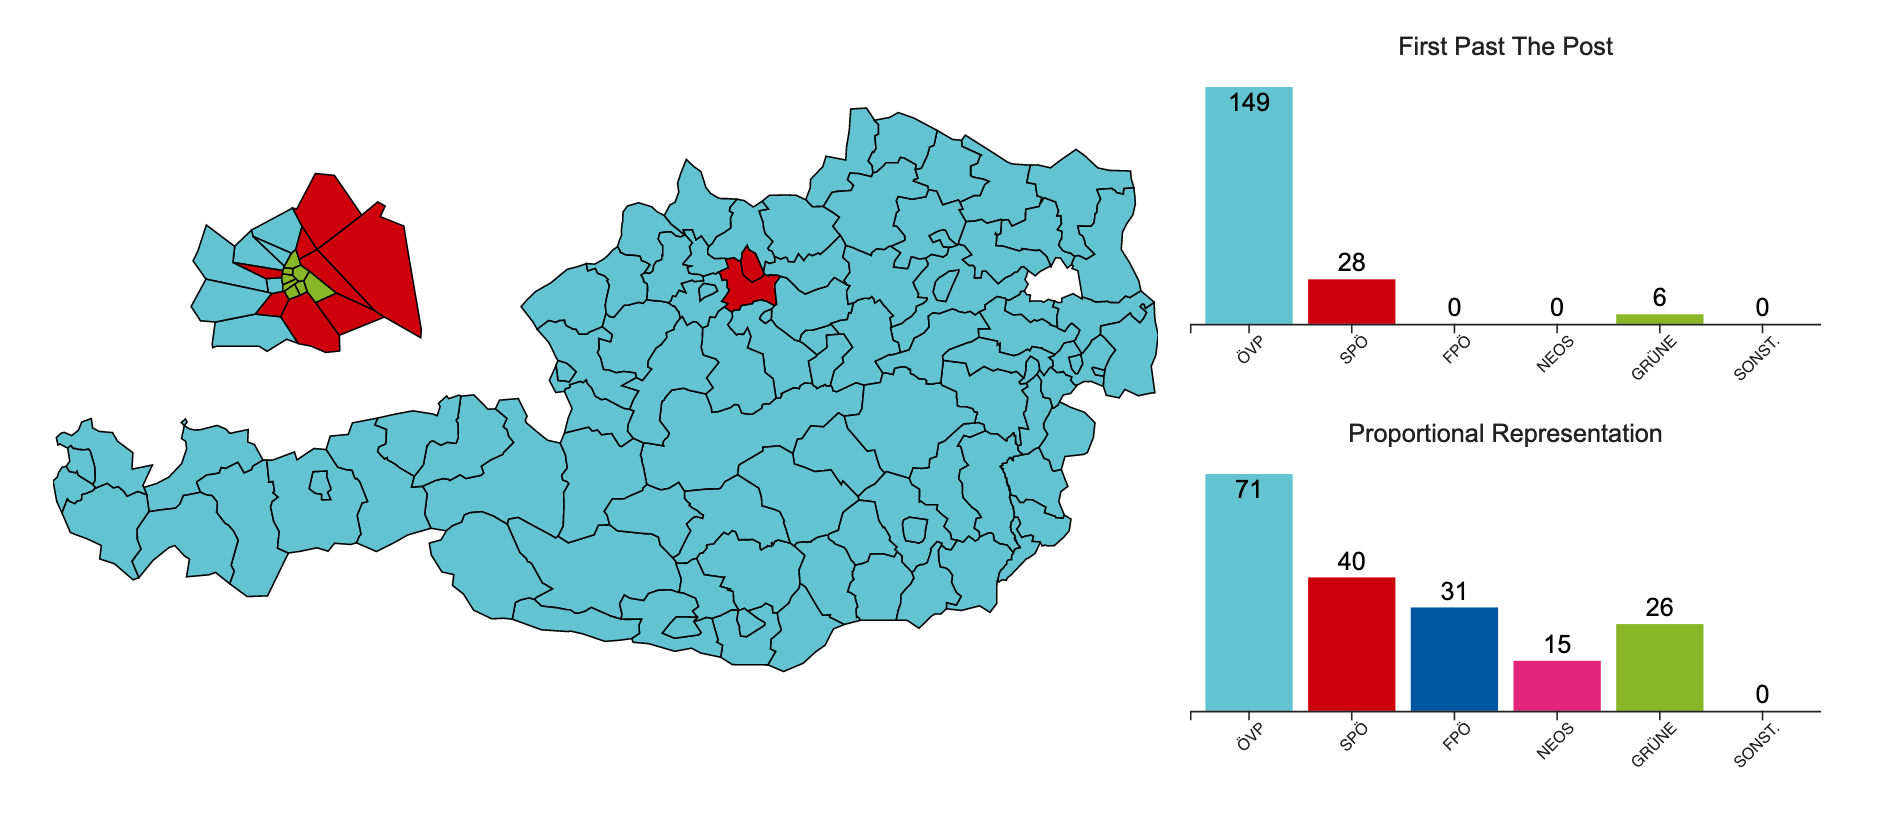
\includegraphics[width=0.9\linewidth]{images/mapbywahlbezirken.png}
  \caption{\label{fig:mapOfResults} Map of Results}
\end{figure}
\end{frame}

\begin{frame}
\frametitle{Takeaway}
\begin{figure}[h]
  \centering
  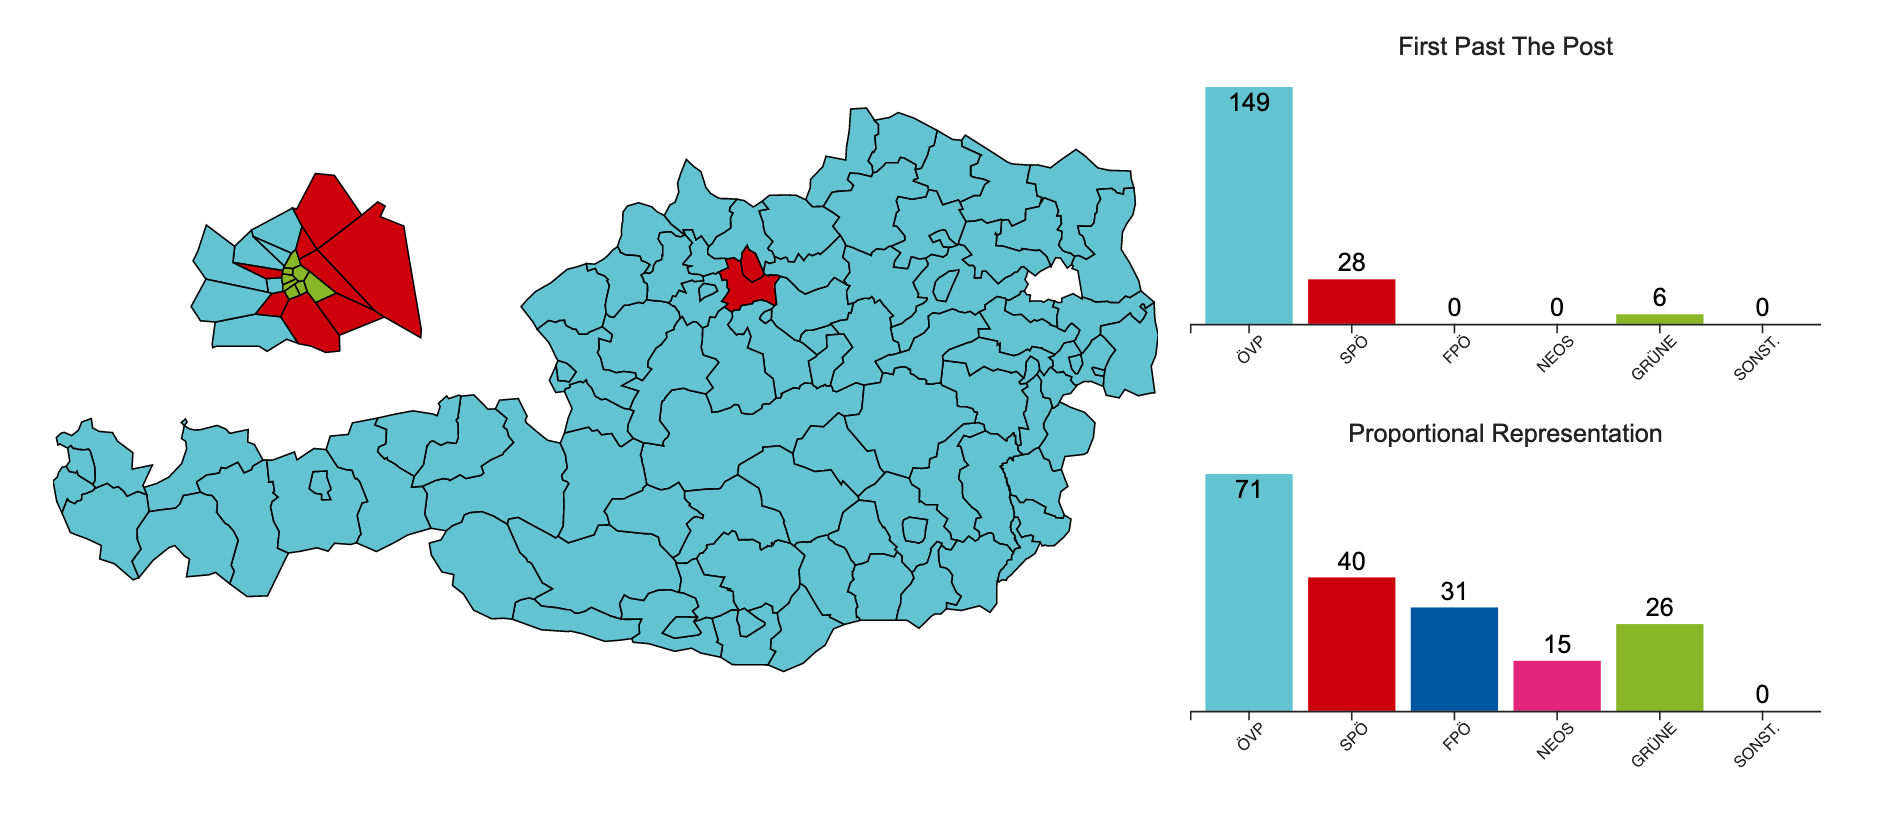
\includegraphics[width=0.9\linewidth]{images/mapbywahlbezirken.png}
  \caption{\label{fig:mapOfResults} Map of Results}
\end{figure}
\begin{itemize}
\item Would result in less party plurality 
\item Hugh wins do not make a difference within one region
\item In Austria: more power for the countryside and less power for capitals
\item No coalition government 
%\item It would never have made a difference if I would have cast a vote or not. 
\end{itemize}
\end{frame}


\begin{frame}
% Dumb slide maybe we take this one out?
\frametitle{Outlook to future work}
\begin{itemize}
\item Make graphics more user mobile-friendly 
\item Compare more years
\item Compare Austrian presidential elections to US presidential elections
\item Check how many votes the winning party could lose and still govern alone (50\% + 1) and change the constitution on their own (66,67\%).
\end{itemize}
\end{frame}

\begin{frame}
%\Huge{\centerline{The End}}
\centerline{L. da Cunha Melo \& S. Reisinger}
\frametitle{Thank you for your attention!}
\begin{figure}
    \centering
    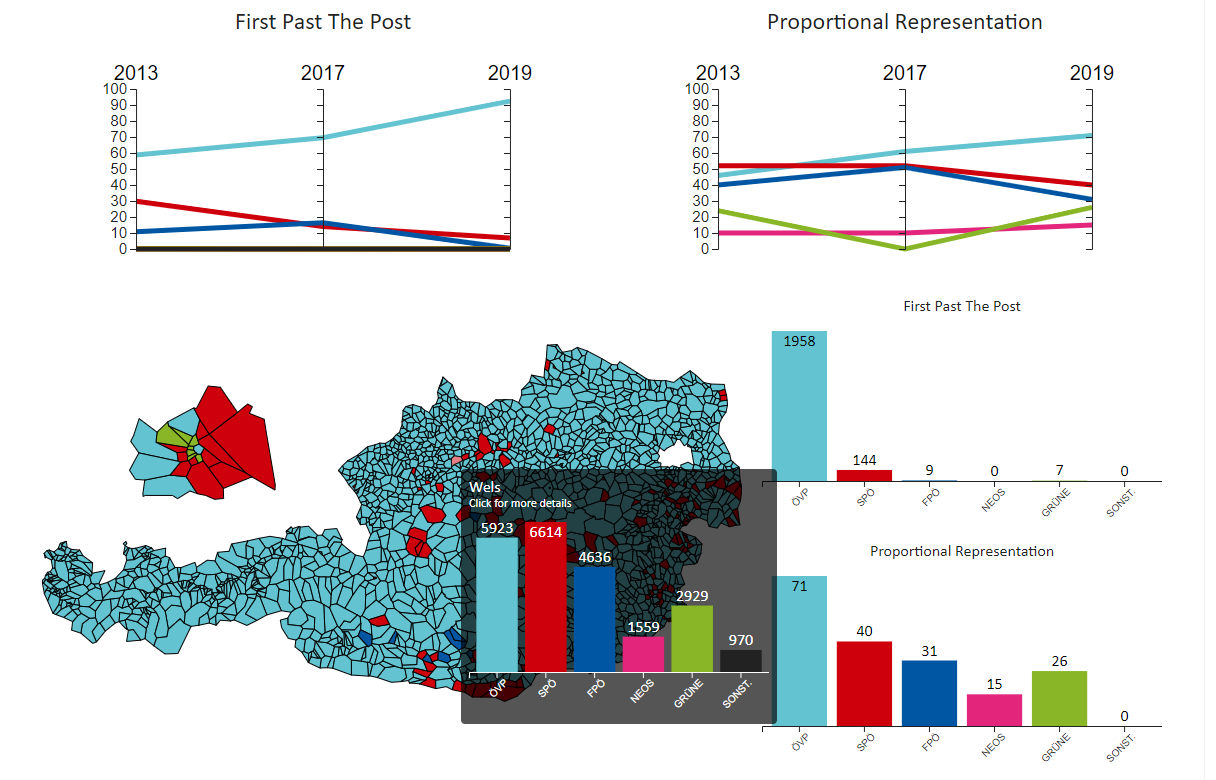
\includegraphics[width=0.9\textwidth]{images/screenshot.png}
\end{figure}

\end{frame}

%----------------------------------------------------------------------------------------

\end{document}